% Fig 2.4 -- cdf of a fair die, jump 1/6 at every face value (web-original
%             figure, no manuscript tikzpicture; redrawn 2026-08-02 to
%             replace the hand-written SVG, which carried Chinese labels and
%             collided the y tick with the axis name)
% Same x range and tick scheme as Fig 2.3 (dice-pmf-threshold.tex);
% same y scale as Fig 2.5 (two-ball-sum-cdf.tex): y=3 is the probability 1.
\documentclass[tikz,border=2pt]{standalone}
\usepackage{amsmath}
\usepackage{amssymb}
\usepackage{xcolor}
\usetikzlibrary{arrows.meta}
\newcommand{\sssig}{\scriptscriptstyle}

\definecolor{journalink}{HTML}{1F1C18}
\definecolor{journalmuted}{HTML}{8A7F72}
\definecolor{journalaccent}{HTML}{9C2D2D}

\begin{document}
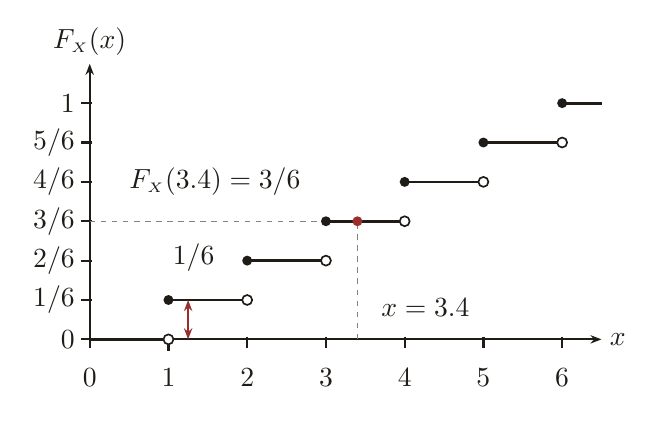
\begin{tikzpicture}[
  x=1cm,
  y=1cm,
  every node/.style={font=\normalsize, journalink},
  axis/.style={journalink, line width=0.8pt, -{Stealth[length=4pt]}},
  tick/.style={journalink, line width=0.8pt},
  stepline/.style={journalink, line width=1.0pt},
  guide/.style={journalmuted, line width=0.5pt, dash pattern=on 2pt off 2pt},
  jump/.style={journalaccent, line width=0.8pt,
               {Stealth[length=4pt]}-{Stealth[length=4pt]}},
  solidpt/.style={circle, fill=journalink, inner sep=0pt, minimum size=3.6pt},
  openpt/.style={circle, draw=journalink, line width=0.6pt, fill=white,
                 inner sep=0pt, minimum size=3.6pt},
  accentpt/.style={circle, fill=journalaccent, inner sep=0pt,
                   minimum size=3.6pt}
]
  % ---- axes ----
  \draw[axis] (0,0) -- (6.5,0);
  \draw[axis] (0,0) -- (0,3.5);

  % ---- x ticks (the tick at x=1 is lengthened to clear the open endpoint) ----
  \foreach \x in {0,2,3,4,5,6}
    \draw[tick] (\x,0.035) -- (\x,-0.106);
  \draw[tick] (1,0.035) -- (1,-0.150);
  \foreach \x in {0,1,2,3,4,5,6}
    \node[anchor=north] at (\x,-0.25) {$\x$};

  % ---- y ticks: y=3 corresponds to the probability 1 ----
  \foreach \y/\lab in {0.5/1, 1/2, 1.5/3, 2/4, 2.5/5}
    \draw[tick] (0.035,\y) -- (-0.106,\y)
      node[anchor=east, inner sep=2pt] {$\lab/6$};
  \draw[tick] (0.035,0) -- (-0.106,0) node[anchor=east, inner sep=2pt] {$0$};
  \draw[tick] (0.035,3) -- (-0.106,3) node[anchor=east, inner sep=2pt] {$1$};

  % ---- guides locating the value at the threshold 3.4 ----
  \draw[guide] (0,1.5)   -- (3,1.5);
  \draw[guide] (3.4,0) -- (3.4,1.5);

  % ---- step segments ----
  \draw[stepline] (0,0)   -- (1,0);
  \draw[stepline] (1,0.5) -- (2,0.5);
  \draw[stepline] (2,1)   -- (3,1);
  \draw[stepline] (3,1.5) -- (4,1.5);
  \draw[stepline] (4,2)   -- (5,2);
  \draw[stepline] (5,2.5) -- (6,2.5);
  \draw[stepline] (6,3)   -- (6.5,3);

  % ---- jump height at the first face value ----
  \draw[jump] (1.25,0) -- (1.25,0.5);
  \node[anchor=south] at (1.32,0.74) {$1/6$};

  % ---- endpoints (drawn last, on top of the segments) ----
  \node[openpt]  at (1,0)   {};
  \node[solidpt] at (1,0.5) {};
  \node[openpt]  at (2,0.5) {};
  \node[solidpt] at (2,1)   {};
  \node[openpt]  at (3,1)   {};
  \node[solidpt] at (3,1.5) {};
  \node[openpt]  at (4,1.5) {};
  \node[solidpt] at (4,2)   {};
  \node[openpt]  at (5,2)   {};
  \node[solidpt] at (5,2.5) {};
  \node[openpt]  at (6,2.5) {};
  \node[solidpt] at (6,3)   {};

  % ---- the value at the threshold ----
  \node[accentpt] at (3.4,1.5) {};
  \node[anchor=south west] at (0.38,1.70) {$F_{\sssig X}(3.4)=3/6$};
  \node[anchor=west] at (3.58,0.40) {$x=3.4$};

  % ---- axis labels ----
  \node[anchor=west, inner sep=0pt] at (6.6,0) {$x$};
  \node[anchor=south, inner sep=0pt] at (0,3.6) {$F_{\sssig X}(x)$};
\end{tikzpicture}
\end{document}
